\documentclass[a4paper, 12pt]{article}

\usepackage{graphicx} % Required for inserting images
\usepackage{setspace}
\usepackage{geometry}
\usepackage{float}
\usepackage[polish]{babel}
\usepackage[T1]{fontenc}

\usepackage[
     backend=biber,
]{biblatex}
\addbibresource{sources.bib}

\geometry
{
     top=1.5cm,
     bottom=2cm,
     left=2cm,
     right=2cm,
}
\linespread{1.1}


\begin{document}

\vspace*{\fill}

PLACEHOLDER

\vspace*{\fill}

\newpage

\section{Wstęp}

\section{Parametry opisujące jakość powietrza}

Pomimo spadającej liczby śmierci spowodowanych niską jakością powietrza 
wewnętrznego, co sugeruje ogólną poprawę jakości powietrza, nie można 
stwierdzić wyeliminowania tego problemu. Na całym świecie aż 4\% wszystkich 
zgonów przypisuje się właśnie zanieczyszczeniom powietrza wewnętrznego. 
Szczególnie narażone są kraje biedne i mniej rozwinięte technologicznie \cite{owid}.

Pomijając tak drastyczne przypadki zła kondycja powietrza może powodować szereg mniej 
groźnych problemów zdrowotnych, takich jak pogorszenie zdolności rozwiązywania 
problemów i podejmowanie decyzji \cite{co2-effects}, co w szczególności dotyka placówki oświatowe i 
osoby tam przebywające. 

Bacząc na powyższe, oraz na fakt że człowiek średnio spędza większość dnia w swoim 
domu \cite{time-indoors}, nie licząc takich aktywności jak praca w zamkniętym pomieszczeniu, nowoczesne 
budynki powinny umożliwiać monitorowanie stanu powietrza wewnątrz 
ich w celu lepszej kontroli nad ich jakością.

Stan jakości powietrza wewnętrznego można opisać szeregiem parametrów: przepływ powietrza, 
pomiar stężenia cząsteczek stałych, tlenków węgla czy dwutlenku siarki. Jednymi z 
najczęściej stosowanych parametrów są jednak temperatura, wilgotność powietrza oraz 
zawartość dwutlenku węgla w powietrzu. 

\subsection{Temperatura}

Komfortowy przedział temperatur dla człowieka w zamkniętych pomieszczeniach w dużej 
mierze zależy od otaczającego klimatu i przyzwyczajeń z tego wynikających. Zależy on od takich czynników 
jak wiek, płeć, pora roku, klimat na danym obszarze czy rodzaj wykonywanej pracy.

W Polsce za minimalną dopuszczalną temperaturę w miejscu pracy przyjmuje się 18st. Celsjusza dla 
lekkiej pracy niewymagającej wysiłku fizycznego oraz 14st. dla pomieszczeń, w których wykonywane są prace 
fizyczne \cite{manutan-bhp}. Aktualne przepisy BHP nie normują jednak maksymalnej dopuszczalnej temperatury. 
Kolejnym dokumentem pomagającym przybliżyć komfortowy przedział temperatur w pomieszczeniach jest
"Rozporządzenie Min. Infrastruktury z 12.04.2002 w sprawie warunków technicznych jakim powinny odpowiadać 
budynki i ich usytuowanie", a dokładnie art. 134 punkt 2 \cite{rozp-bud}. Określono tam temperaturę na potrzeby obliczeń szczytowej 
mocy cieplnej w pomieszczeniach zależnie od ich przeznaczenia.
Dla przykładu, pomieszczenia przeznaczone na stały pobyt ludzi bez okryć zewnętrznych, niewykonujących 
w sposób ciągły pracy fizycznej posiadają temperaturę obliczeniową 20st.C:

Potocznie zaś dla zastosowań codziennych przyjmuje się przedział 18-22 st.C.

Za niska temperatura może powodować zwiększoną śmiertelność z powodu chorób układu oddechowego czy podwyższone 
ciśnienie \cite{who-cold}. Za wysoka zaś oprócz oczywistego dyskomfortu może doprowadzić zwiększonej śmiertelności, 
szczególnie u osób z chorobami układu oddechowego czy cierpiących na arytmię \cite{bmj-heat}

\subsection{Wilgotność}

Wilgotność powietrza można mierzyć na parę sposobów, natomiast odpowiednie aspekty tej pracy będą 
skupiały na wilgotności względnej - jest to stosunek wilgotności bezwzględnej powietrza do jej wartości 
maksymalnej w danej temperaturze \cite{termodynamika}

W pomieszczeniach biurowych o regulowanej temperaturze za optymalny zakres przyjmuje się 
od 25 do 60 \% wilgotności \cite{inz-bud}. Niższa wilgotność, szczególnie w połączeniu z niską temperaturą 
mogą przyczyniać się do zwiększonego występowania chorób układu oddechowego \cite{low-hum}. Za wysoka wilgotność 
zaś sprzyja rozwojowi i rozprzestrzenianiu się związków biologicznych (bakterie, wirusy, grzyby) 
powodujących alergie i choroby zakaźne \cite{high-hum}.

Podobnie jak temperatura, wilgotność zależy od wielu czynników i może zmieniać się bardzo dynamicznie, 
nawet w ciągu dnia. Wpływanie na wilgotność powietrza polega przede wszystkim na możliwości odczytu 
jego aktualnej lub historycznej wartości.

\begin{figure}[!h]
    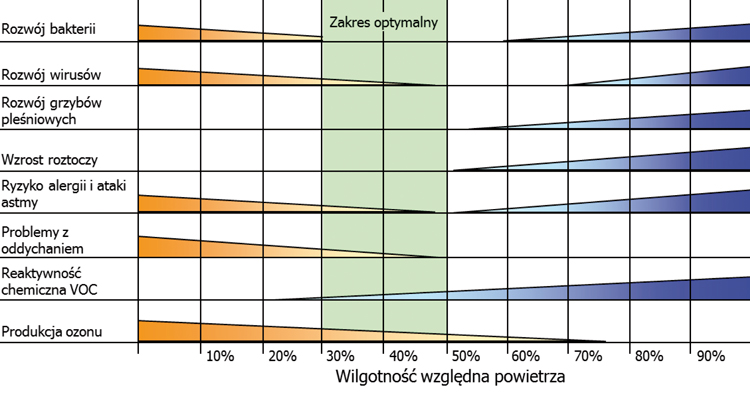
\includegraphics[width=\textwidth]{zdj/wilgotnosc_powietrza_w_pomieszczeniach.jpg}
    \caption{Wpływ wilgotności powietrza na nasilenie poszczególnych czynników}
\end{figure}

\subsection{Dwutlenek węgla}

Podobnie jak w przypadku wilgotności, zawartość CO2 w powietrzu można mierzyć w wielu jednostkach. 
W tej pracy zdecydowano się jednak posługiwać się jednostką ppm - części na milion.

Za standard bezpiecznego poziomu CO2 w pomieszczeniu przyjmuje się wskaźnik Pettenkofera, który określa, 
że bezpieczne maksymalne stężenie tego związku w powietrzu wyrażone w częściach na milion wynosi 1000ppm \cite{pettenhofer}.

Rozporządzenie ministra rodziny, pracy i polityki społecznej z dnia 12 czerwca 2018 r. w sprawie 
najwyższych dopuszczalnych stężeń i natężeń czynników szkodliwych dla zdrowia w środowisku \cite{min-stezenia} pracy określa 
dopuszczalne stężenia szkodliwych dla człowieka substancji w trakcie pracy. Dla CO2 jest to:

* 9000 mg/m3 (~4,917ppm) - wartość średnia ważona, w ciągu 8-godzinnego dobowego i przeciętnego tygodniowo wymiaru pracy
* 27000 mg/m3 (~14,752ppm) - maksymalne stężenie, które może występować nie dłużej niż 15min, nie częściej niż 2 razy w ciągu zmiany i w odstępie dłuższym niż 1 godzina.

Standardowa ilość atmosferycznego dwutlenku węgla w powietrzu wynosi aktualnie około 417ppm. 
Liczba ta od początku Rewolucji Przemysłowej w 1750r. stale rośnie \cite{atmo-co2-change}, a według niektórych danych jest 
ono nawet 50\% wyższe niż sprzed wspomnianej daty \cite{50-percent}. Stężenie CO2 w powietrzu wyższe od 
wspomnianego wskaźnika Pettenkofera może powodować trudności w koncentracji, senność czy 
trudności z oddychaniem \cite{pettenhofer}.

\begin{figure}
    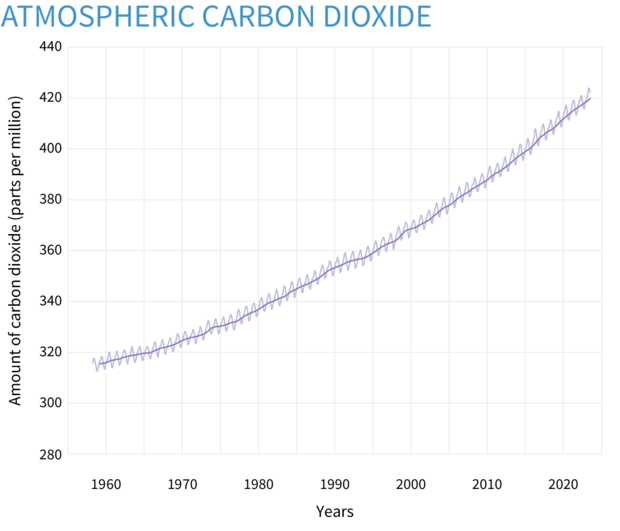
\includegraphics[width=\textwidth]{zdj/more-co2.png}
    \caption{Wzrost stężenia dwutlenku węgla w atmosferze na przestrzeni lat}
\end{figure}

\section{Bezprzewodowy system monitoringu parametrów jakości powietrza}

\subsection{Technologia IQRF}

IQRF jest to bezprzewodowa technologia Mesh pracująca w pod-gigaherzowych pasmach ISM. Nie wymaga żadnej zewnętrznej infrastruktury, 
licencji i opłat dostawcy \cite{what-iqrf}. Zamontowanie transceivera IQRF w kompatybilnych urządzeniach pozwala im na komunikację między sobą
poprzez przesyłanie pakietów danych. 

Każda sieć wykorzystująca IQRFMESH potrzebuje koordynatora do odpowiedniego działania. Urządzenia w sieci komunikują się na zasadzie
master(koordynator) - slave(węzeł). Węzły nie mogą komunikować się ze sobą bezpośrednio, natomiast w topologi innej niż
Gwiazda (np. Mesh) węzły wspierają routowanie pakietów do innych węzłów \cite{iqrf-rules}.

IQRFMESH jest protokołem umożliwiającym, między innymi, zwiększenie zasięgu sieci poprzez umożliwienie węzłom routowania pakietów.
Jest możliwe połączenie urządzeń bez wykorzystania tego protokołu, ale na potrzeby tej pracy jest to silnie zalecane. \cite{iqrfmesh} Urządzenia w 
sieci IQRFMESH komunikują się poprzez protokół DPA, w której wiadomości są przesyłane w strukturze bajtowej \cite{dpa-guide}.

[PRZYKŁAD WIADOMOŚCI]

\subsection{Czujniki i bramka IQRF}

Urządzeniami bezpośrednio odpowiedzialnymi za pobieranie z otoczenia danych o jakości powietrza są cztery czujniki NLB-CO2+RH+T-5-IQRF.
Każdy czujnik jest w stanie odczytać temperaturę, wilgotność względną oraz zawartość dwutlenku węgla w powietrzu. Zasilanie jest zapewniane
bateryjnie poprzez dwie baterie AA 1.5V, a komunikacja odbywa się poprzez zamontowany w gnieździe nadajnikoodbiornik (transceiver) IQRF
zamontowany w gnieździe SIM. Każdy taki sensor stanowi węzeł sieci IQRFMESH.

[JAKIEŚ ZDJĘCIE]

Koordynatorem sieci jest bramka GW-ETH02 zasilana sieciowo napięciem 5VDC. Urządzenie łączy się z Internetem poprzez gniazdo Ethernet oraz
posiada gniazdo karty SD jako jedną z opcji zapisu danych. Bramka posiada wbudowany transceiver IQRF.

[ZDJ]

TUTAJ NAPISZ O SAMYCH KOSTKACH IQRF - WERSJE OS, DPA, ETC.

\subsubsection{Konfiguracja czujników}

PYTANIE: czy transceivery IQRF trzeba było dodatkowo konfigurować, czy one w ogóle były w zestawie z czujnikami?
ODP.: W dokumentacji protronixa mamy "The factory produces IQRF modules in sensors with the following configuration:" więc założę, że
mamy w zestawie i skonfiguroane

Do konfiguracji urządzeń wchodzących w skład sieci posłużono się narzędziem IQRF IDE w wersji 4.70. Narzędzie to umożliwia między 
innymi konfigurację modułów IQRF TR zawartych w urządzeniach oraz odczyt pewnych danych o transceiverach IQRF, takich jak wersja 
ssy 

Bramka datalogger

\subsection{Serwer IQRF Cloud}

IQRF Cloud jest serwisem w chmurze umożliwiającym komunikację z bramką IQRF po jej zarejestrowaniu w tymże serwisie, w którym uprzednio należy
założyć konto. Po rejestracji serwis umożliwia obustronną komunikację z urządzeniem w postaci wiadomości protokołu DPA. Aby takową nadać należy 
wejść w panel zarejestrowanej bramki i wybrać opcję "Send data to gateway":

[OPCJA]

Po wybraniu tej opcji otrzymujemy widok umożliwiający wysyłanie do brami wiadomości protokołem DPA, a każde nadanie wymaga dodatkowo podania
hasła do bramki wybieranego na etapie konfiguracji

[EKRAN NADAWANIA WIADOMOŚCI]

Dane odbierane/wysyłane przez serwer i bramkę są widoczne w panelu głównym odpowiednim dla bramki. Każdy rekord składa się z indeksu, czasu
otrzymania przez serwer i bramkę, kierunku przesyłu danych (transmisja a odbiór), długości przesłanych danych w bajtach, przesłanych danych
w postaci ciągu znaków 0-9 A-F 

Każdy rekord skład się z:
\begin{itemize}
    \item indeksu 
    \item czasu otrzymania przez serwer i bramkę
    \item kierunku przesyłu danych (transmisja a odbiór)
    \item długości danych wyrażonej w bajtach 
    \item samych danych w formacie szesnastkowym (znaki 0-9 i A-F)
    \item statusu odebrania przez bramkę (Sent, Confirmed, Expired...)
    \item indeksu w bazie danych serwera.
\end{itemize}

Powyższy panel jednak stanowi dla tej pracy bardziej narzędzie diagnostyczne niż kluczowy element działania systemu - z poziomu działania aplikacji
webowej nie da się wejść w interakcję z tym panelem, a przynajmniej nie jest to przewidziane. Serwis udostępnia więc własny interfejs 
programistyczny (API), który umożliwia przesyłanie zapytań z innego urządzenia do tego serwisu i w konsekwencji do bramki oraz czujników.

Każde zapytanie wysyłane do serwera składa się z adresu bazowego na jaki przesyłamy zapytania, wymaganych i opcjonalnych parametrów oraz tzw. 
sygnatury. Adresem bazowym na dzień pisania pracy jest \textbf{https://cloud.iqrf.org/api/api.php?}.

\subsubsection{Parametry wymagane i opcjonalne}

Wyczerpująca lista parametrów wymaganych prezentuje się następująco:

\begin{itemize}
    \item ver - aktualna wersja API. W trakcie pisania pracy jest to "2" 
    \item uid - login użytkownika do serwisu IQRF Cloud
    \item gid - ID zarejestrowanej bramki, z którą chcemy się komunikować. Widoczne zarówno w portalu jak i na obudowie bramki
    \item gpw - hasło do bramki. Wymagane jedynie w przypadku stosowania komendy "add"
    \item cmd - jedna z komend: dnld, uplc, dnlc
    \item data - dane do przesłania do bramki
    \item signature - podpis potwierdzający użytkownika.
\end{itemize}

Parametry opcjonalne dają kontrolę nad ilością pobieranych danych. Lista wyczerpująca:

\begin{itemize}
    \item from - indeks pierwszego rekordu, który chcemy pobrać
    \item to - indeks ostatniego rekordu, który chcemy pobrać
    \item count - ilość pobieranych rekordów
    \item time\_from - data utworzenia pierwszego rekordu, który chcemy pobrać 
    \item time\_to - data utworzenia ostatniego rekordu, który chcemy pobrać
    \item new - pobieranie danych zaczynając od ostatniego pobranego rekordu
    \item last - pobieranie rekordów zaczynając od najpóźniejszych
\end{itemize}

Bardziej szczegółowy opis wszystkich parametrów oraz ograniczenia w ich stosowaniu dostępne są w dokumentacji IQRF Cloud Serwer Technical Guide 
\cite{iqrfcloud-guide}

\subsubsection{Sygnatura zapytania}

Jakakolwiek komunikacja z serwerem wymaga podaniu parametru \textbf{signature}, który gwarantuje bezpieczeństwo przesyłu danych przez API 
potwierdzając prawo dostępu użytkownika do danych. Dokumentacja \cite{iqrfcloud-guide} definiuje sygnaturę następująco:

[ZDJ MD5]

Gdzie: 

\begin{itemize}
    \item parameter\_part - ciąg znaków adresu URL zapytania pomiędzy adresem bazowym a sygnaturą. Na przykład, dla zapytania \\
"https://cloud.iqrf.org/api/api.php?ver=2\&uid=xxx\&gid=xxx\&cmd=dnld\&signature=xxx" \\ 
wartość ta jest równa "ver=2\&uid=xxx\&gid=xxx\&cmd=dnld"
    \item api\_key - klucz API dostępny po zalogowaniu się do portalu IQRF Cloud
    \item ip\_address - adres IP klienta
    \item timestamp - liczba sekund począwszy od 01.01.1970 00:00UTC podzielona przez 600. Podzielenie przez 600 zapewnia 10-minutową
ważność każdej sygnatury.
\end{itemize}

"md5" jest zaś kryptograficzną funkcją haszującą. 

[ZDJĘCIE KLUCZA API Z PANELU]

\section{Bibliografia}

\printbibliography

\end{document} 